\documentclass[tikz,border=10pt]{standalone}
\begin{document}
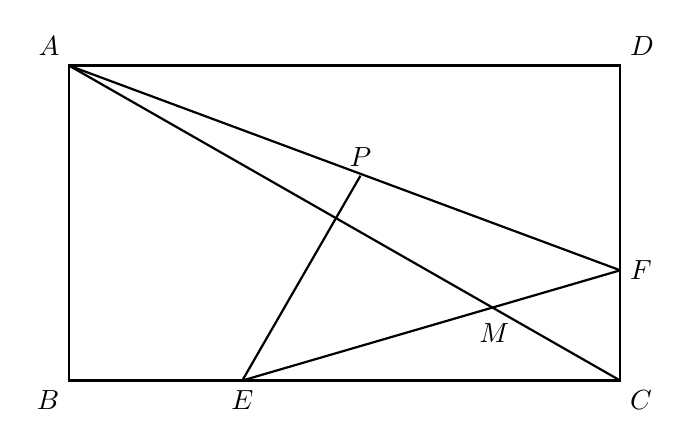
\begin{tikzpicture}[scale=1]
\coordinate (A) at (0,4);
\coordinate (B) at (0,0);
\coordinate (C) at (7,0);
\coordinate (D) at (7,4);
\coordinate (E) at (2.2,0);
\coordinate (F) at (7,1.4);
\coordinate (P) at (3.7,2.6);
\coordinate (M) at (5.4,0.85);

\draw[thick] (A) -- (B) -- (C) -- (D) -- cycle;
\draw[thick] (A) -- (C);
\draw[thick] (A) -- (F);
\draw[thick] (E) -- (F);
\draw[thick] (P) -- (E);
\draw[dashed] (P) -- (E);

\node[above left] at (A) {$A$};
\node[below left] at (B) {$B$};
\node[below right] at (C) {$C$};
\node[above right] at (D) {$D$};
\node[below] at (E) {$E$};
\node[right] at (F) {$F$};
\node[above] at (P) {$P$};
\node[below] at (M) {$M$};
\end{tikzpicture}
\end{document}
